\documentclass[hidelinks,aspectratio=169]{beamer}
\usepackage[italian]{babel} 
\usepackage[utf8]{inputenc} 
\usepackage{fourier} 


%Slide colors
\usetheme{Boadilla}
\usecolortheme{beaver}

% Images
\usepackage{graphicx}
\usepackage{caption}
\usepackage{subcaption}
\usepackage{float}
\graphicspath{ {../Images} }

% FlowChart
\usepackage{smartdiagram}

% Stop hyphenation
\usepackage[none]{hyphenat}

% Coloring links
\usepackage{xcolor}

% Enumerate abc
\usepackage{enumerate}

% Minipages in the same line
\usepackage{tabularx}

% License
\usepackage[
type={CC},
modifier={by-nc-sa},
version={4.0},
]{doclicense}

% Command to enumerate frames title
\newcommand{\numcirc}[1]{%
	%   \usebeamerfont*{item projected}%
	\large
	\usebeamercolor[bg]{item projected}%
	\begin{pgfpicture}{-1ex}{0ex}{1ex}{2ex}
		\pgfpathcircle{\pgfpoint{0pt}{.75ex}}{1.2ex}
		\pgfusepath{fill}
		\pgftext[base]{\color{fg}#1}
	\end{pgfpicture}%
	\usebeamerfont*{frametitle}%
}

%Command to zoom in
\usepackage{mwe}
\makeatletter
\newsavebox\zb@x
\newcounter{z@@m}
\usepackage{calc}
\newdimen\B@r\newdimen\P@r
\newdimen\@zw\newdimen\@zh\newdimen\@zd

\newcommand{\zoombox}[2][0]{%
	\leavevmode%
	\sbox\zb@x{#2}%
	\setlength\B@r{1pt*\ratio{\wd\zb@x}{\ht\zb@x+\dp\zb@x}}%
	\setlength\P@r{1pt*\ratio{\paperwidth}{\paperheight}}%
	\ifdim\B@r>\P@r\relax%
	\setlength\@zw{\wd\zb@x}\setlength\@zh{\@zw*\ratio{\paperheight}{\paperwidth}}%
	\setlength\@zd{(\@zh-\ht\zb@x-\dp\zb@x)*\real{0.5}+\dp\zb@x}%
	\setlength\@zh{\@zh-\@zd}%
	\else%
	\setlength\@zh{\ht\zb@x+\dp\zb@x}%
	\setlength\@zw{\@zh*\ratio{\paperwidth}{\paperheight}}%
	\setlength\@zh{\ht\zb@x}\setlength\@zd{\dp\zb@x}%
	\fi%
	\makebox[0pt][l]{\makebox[\wd\zb@x][c]{\makebox[\@zw][l]{%
				\pdfdest name {zbfs\thez@@m} fitr
				width  \@zw\space
				height \@zh\space
				depth  \@zd\space
	}}}%
	\pdfdest name {zb\thez@@m} fitr
	width  \wd\zb@x\space
	height \ht\zb@x\space
	depth  \dp\zb@x\space
	\immediate\pdfannot 
	width  \wd\zb@x\space
	height \ht\zb@x\space
	depth  \dp\zb@x\space
	{%
		/Subtype/Link/H/N
		/Border [0 0 #1 [1 2]]
		/A <<
		/S/JavaScript
		/JS (
		if(typeof(zoomed)=='undefined'||!zoomed){
			var lastView=this.viewState;
			if(app.fs.isFullScreen) this.gotoNamedDest('zbfs\thez@@m');
			else this.gotoNamedDest('zb\thez@@m');
			zoomed=true;
		}else{
			this.viewState=lastView;
			zoomed=false;
		}
		)
		>>
	}%
	\usebox{\zb@x}%
	\stepcounter{z@@m}%
} 
\makeatother



%Header
\title[Identità e valore della stampa d'arte]{\textbf{Identità e valore della stampa d'arte}}
\author{Roberto Budassi}
\date{}

\begin{document}
	
		\begin{frame}
		\maketitle
		
		\vspace*{\fill}
		\centering
		\fboxrule=2pt
		\fbox
		{
			\begin{minipage}{0.9\linewidth}
				\small{Il seguente documento è ottimizzato per la visualizzazione digitale con \href{https://get.adobe.com/it/reader/}{\textcolor{blue}{Adobe~Acrobat~Reader}}.}  
			\end{minipage}
		}
	\end{frame}
	
	\begin{frame}
		\tableofcontents
	\end{frame}
	
	\section{Sul concetto di \textbf{originalità} e \textbf{autenticità}}
	\begin{frame}{Sul concetto di \textbf{originalità} e \textbf{autenticità}}
		\begin{itemize}
			\item 1937	Parigi: Exposition Internationale - Comité National de la Gravure
			\item 1960	Vienna: 3° Congresso - Associazione Internazionale delle Arti Plastiche
			\item 1961	New York: Print Council of America
			\item 1964	Parigi: Comité International de la Gravure
			\item 1991	Venezia: convegno organizzato dalla Biennale di Venezia
			\item 1994	Milano: dichiarazione sull’incisione originale
		\end{itemize}
	\end{frame}
	
	\begin{frame}{Sul concetto di \textbf{originalità} e \textbf{autenticità}}
		In sintesi….“Un’incisione è considerata “originale” quando rispetta le due seguenti caratteristiche:
		\begin{enumerate}[a.]
			\item In fase di stampa dà luogo a un’immagine che deriva da una matrice manualmente incisa (anche nel caso in cui l’artista si sia servito di una base ottenuta con altri procedimenti), o predisposta sempre manualmente dallo stesso artista, con esclusione di qualsiasi mezzo fotomeccanico, allo scopo di essere impressa con intenti estetici.
			\item L’immagine incisa sulla matrice deve seguire la sintassi linguistica propria dell'incisione, e cioè un appropriato e intenzionale uso delle tecniche specifiche.
		\end{enumerate}
		Per analogia una litografia viene considerata “stampa originale” quando la sua immagine è impressa da una matrice manualmente disegnata o dipinta, allo scopo di essere stampata con intenti estetici.\\
		Qualunque stampa che riproduca un modello, ottenuta con mezzi fotomeccanici, o con altri mezzi non manuali, di qualsivoglia tipo, non può essere chiamata “originale” (e neppure “originaria” o “litografia autentica”).
	\end{frame}
	
	\subsection{Le tecniche originali}
	\begin{frame}{Le tecniche originali}
		Stampa in rilievo (xilografia), in incavo (calcografia), in piano (litografia)
		\begin{tabularx}{\textwidth}{XXX}
			{
			\begin{center}
				\large{Xilografia}\\
				\bigskip
				\begin{itemize}
					\item \small{\textbf{Bulino} su legno di filo}
					\item \small{\textbf{Bulino} su legno di testa}
					\item \small{\textbf{Camaieu}}
					\item \small{\textbf{Criblèe} su metallo}
					\item \small{\textbf{Sgorbia} su linoleum}
					\item \small{\textbf{Sgorbia} su cartone}
				\end{itemize}
			\end{center}
			}&{
			\begin{center}
				\large{Calcografia}\\
				\normalsize
				\bigskip
				\normalsize{(Maniera diretta)}\\
				\begin{itemize}
					\item \scriptsize{\textbf{Niello}}
					\item \scriptsize{\textbf{Bulino}}
					\item \scriptsize{\textbf{Puntasecca}}
					\item \scriptsize{\textbf{Mezzotinto/Maniera nera}}
					\item \scriptsize{\textbf{Carborundum}}
				\end{itemize}
				\medskip
				\normalsize{(Maniera indiretta)}\\
				\begin{itemize}
					\item \scriptsize{\textbf{Acquaforte}}
					\item \scriptsize{\textbf{Acquatinta}}
					\item \scriptsize{\textbf{Maniera a zucchero}}
					\item \scriptsize{\textbf{Vernice molle}}
				\end{itemize}
			\end{center}
			}&{
			\begin{center}
				\large{Litografia}\\
				\normalsize
				\bigskip
				\begin{itemize}
					\item \small{\textbf{Su matrice di pietra}}
					\item \small{\textbf{Su matrice di zinco}}
					\item \small{\textbf{Cromolitografia}}
				\end{itemize}
			\end{center}
			}
		\end{tabularx}
	\end{frame}
	
	\begin{frame}{Le tecniche originali}
		\begin{tabularx}{\textwidth}{XXX}
			{
			\centering
			\zoombox{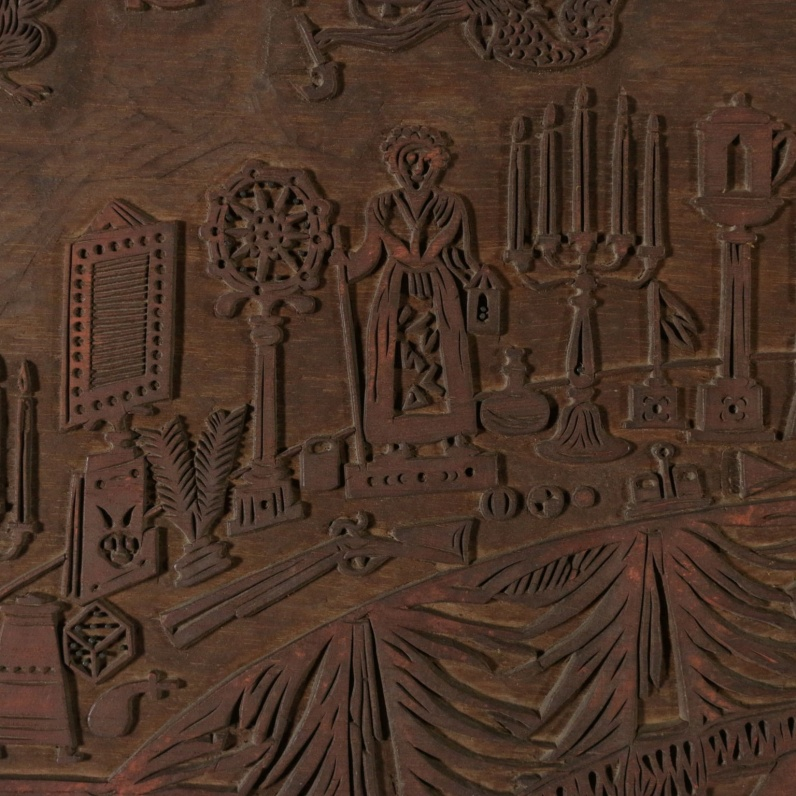
\includegraphics[scale=0.5]{Esempio1.jpg}}
			\captionof{figure}{Esempio 1}
			}&{
			\centering
			\zoombox{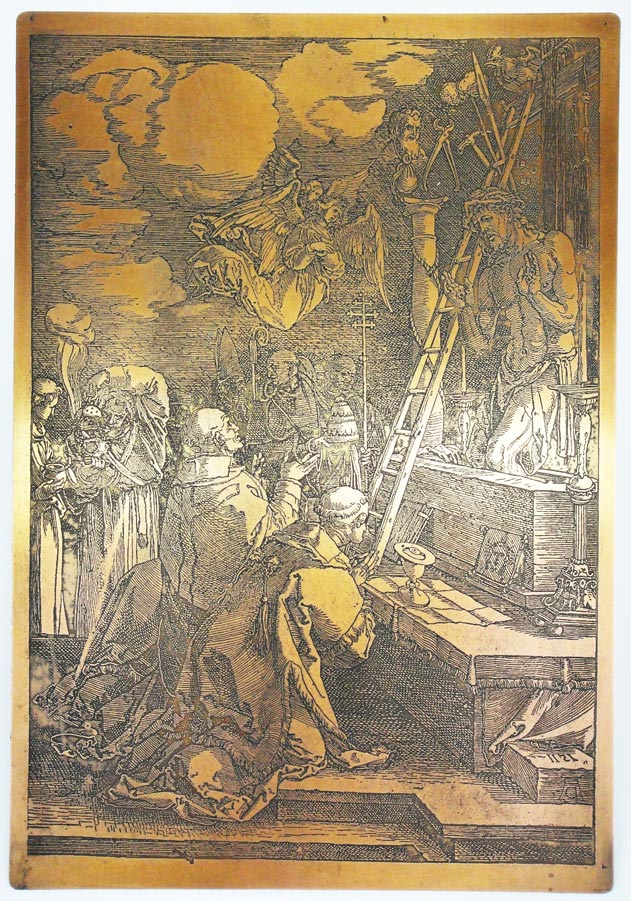
\includegraphics[scale=0.15]{Esempio2.jpg}}
			\captionof{figure}{Esempio 2}
			}&{
			\centering
			\zoombox{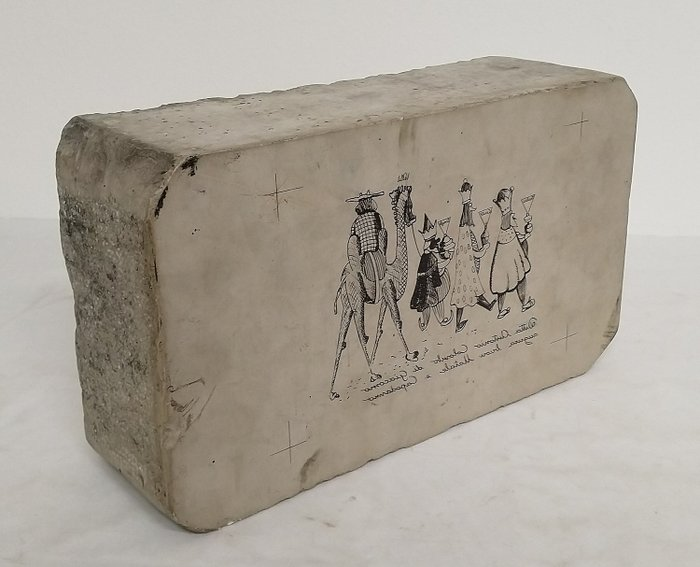
\includegraphics[scale=0.17]{Esempio3.jpg}}
			\captionof{figure}{Esempio 3}
			}
		\end{tabularx}
	\end{frame}
	
	\begin{frame}
		contenuto...
	\end{frame}
	
\end{document}